\documentclass[letterpaper, 11pt]{article}
\usepackage[utf8]{inputenc}
\usepackage[letterpaper, portrait, margin=1in]{geometry}
\usepackage{pgfplots}
\pgfplotsset{width=10cm,compat=1.9}
\usepackage{hyperref}
\usepackage{textcomp}
\usepackage{siunitx}
\usepackage{amsmath}
\usepackage{cancel}
\usepackage{tikz}
\usepackage{everysel}
\usepackage{ragged2e}
\usepackage{mathdots}
\usepackage{yhmath}
\usepackage{color}
\usepackage{array}
\usepackage{multirow}
\usepackage{amssymb}
\usepackage{gensymb}
\usepackage{tabularx}
\usepackage{booktabs}
\usepackage{listings}
\usepackage{xcolor}
\usepackage{enumitem}
\usetikzlibrary{fadings}
\usetikzlibrary{patterns}
\usetikzlibrary{shadows.blur}
\hypersetup{
    colorlinks=true,
    linkcolor=black,
    filecolor=black,      
    urlcolor=blue,
}

\definecolor{codegreen}{rgb}{0,0.6,0}
\definecolor{codegray}{rgb}{0.5,0.5,0.5}
\definecolor{codepurple}{rgb}{0.58,0,0.82}
\definecolor{backcolour}{rgb}{0.95,0.95,0.92}

\lstdefinestyle{mystyle}{
    backgroundcolor=\color{backcolour},   
    commentstyle=\color{codegreen},
    keywordstyle=\color{magenta},
    numberstyle=\tiny\color{codegray},
    stringstyle=\color{codepurple},
    basicstyle=\ttfamily\footnotesize,
    breakatwhitespace=false,         
    breaklines=true,                 
    captionpos=b,                    
    keepspaces=true,                 
    numbers=left,                    
    numbersep=5pt,                  
    showspaces=false,                
    showstringspaces=false,
    showtabs=false,                  
    tabsize=2
}

\lstset{style=mystyle}

\title{COMSC-200 \\ Lab 6}
\author{Ryan Jacoby}
\date{13 October 2020}
\begin{document}

\maketitle

\section{Unique Words}

\begin{lstlisting}[language=c++, caption=main.cpp]
// Ryan Jacoby

#include<iostream>
#include<fstream>
#include<set>
#include<string>

using namespace std;

int main() {
    ifstream fin;
    set<string> fset;
    set<string> duplicates;

    fin.open("input.txt");

    while(fin) {
        string str;
        fin >> str;
        if(fset.find(str) != fset.end()) duplicates.insert(str);
        fset.insert(str);
    }

    set<string>::iterator sit;
    for(sit = duplicates.begin(); sit != duplicates.end(); sit++) fset.erase(*sit);

    for(sit = fset.begin(); sit != fset.end(); sit++) cout << *sit << '\n';

    fin.close();

    return 0;
}
\end{lstlisting}

\begin{lstlisting}[caption=input.txt]
test test2
test2
test3
test2
\end{lstlisting}

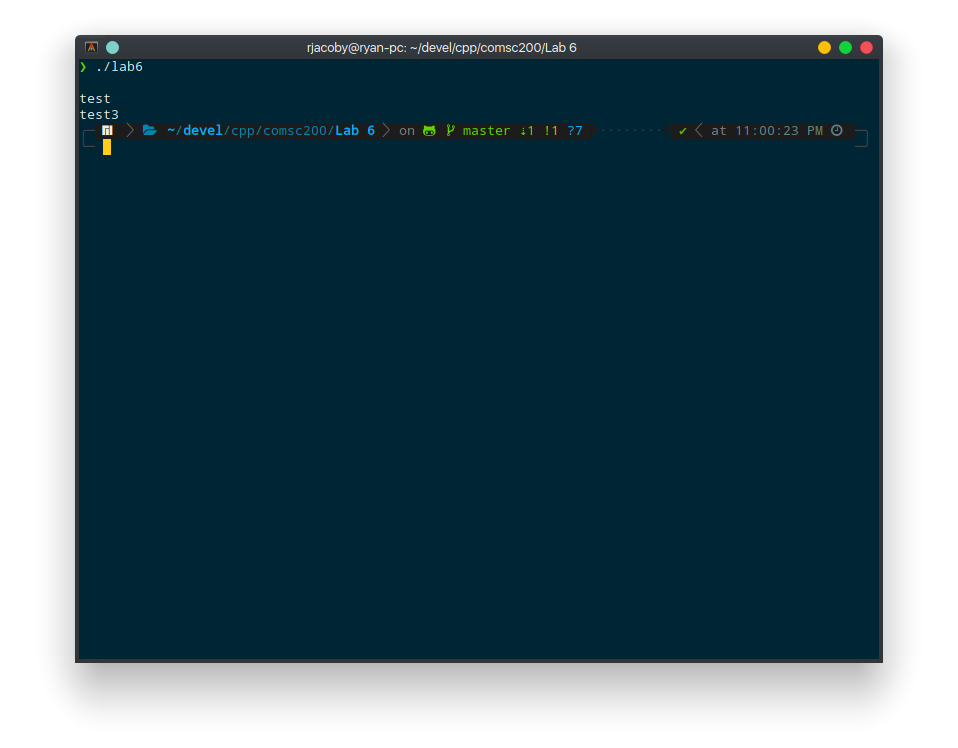
\includegraphics[scale=0.5]{unique.png}

\section{Course Information}

\begin{lstlisting}[language=c++, caption=main.cpp]
// Ryan Jacoby

#include<iostream>
#include<map>

using namespace std;

int main() {
    map<string, int> roomNumber = {{"CS101", 3004}, {"CS102", 4501}, {"CS103", 6755}, {"NT110", 1244}, {"CM241", 1411}};
    map<string, string> instructor = {{"CS101", "Haynes"}, {"CS102", "Alvarado"}, {"CS103", "Rich"}, {"NT110", "Burke"}, {"CM241", "Lee"}};
    map<string, string> meetingTime = {{"CS101", "8:00 a.m."}, {"CS102", "9:00 a.m."}, {"CS103", "10:00 a.m."}, {"NT110", "11:00 a.m."}, {"CM241", "1:00 p.m."}};

    string course;

    cout << "Enter a course number: ";
    cin >> course;

    if(roomNumber.count(course) == 0) cout << "That is not a valid course.\n";
    else cout << course << " meets at " << meetingTime.at(course) << " in room " << roomNumber.at(course) << " and is taught by " << instructor.at(course) << '\n';

    return 0;
}
\end{lstlisting}

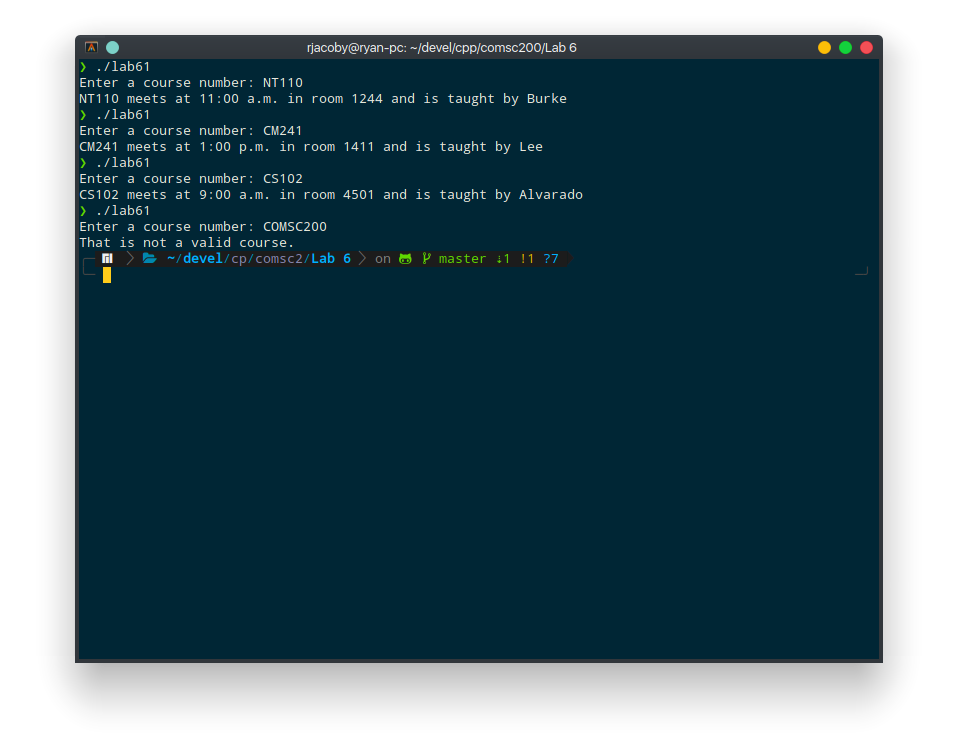
\includegraphics[scale=0.5]{courses.png}

\section{Text File Analysis}

\begin{lstlisting}[language=c++, caption=main.cpp]
// Ryan Jacoby

#include<iostream>
#include<fstream>
#include<set>
#include<string>

using namespace std;

void unique(ifstream *);
void common(ifstream *, ifstream *);
void unique(ifstream *, ifstream *);
void xorFin(ifstream *, ifstream *);

int main() {
    ifstream fin1;
    ifstream fin2;

    fin1.open("input.txt");
    fin2.open("input2.txt");

    cout << "Unique words in file 1:\n";
    unique(&fin1);

    cout << "\nUnique words in file 2:\n";
    unique(&fin2);

    fin1.close();
    fin2.close();
    fin1.open("input.txt");
    fin2.open("input2.txt");

    cout << "\nCommon words between the two files:\n";
    common(&fin1, &fin2);

    fin1.close();
    fin2.close();
    fin1.open("input.txt");
    fin2.open("input2.txt");

    cout << "\nWords that only appear in file 1:\n";
    unique(&fin1, &fin2);

    fin1.close();
    fin2.close();
    fin1.open("input.txt");
    fin2.open("input2.txt");

    cout << "\nWords that only appear in file 2:\n";
    unique(&fin2, &fin1);

    fin1.close();
    fin2.close();
    fin1.open("input.txt");
    fin2.open("input2.txt");

    cout << "\nWords that appear in only one of the files:\n";
    xorFin(&fin1, &fin2);

    return 0;
}

void unique(ifstream *fin) {
    set<string> fset;
    set<string> duplicates;

    while(*fin) {
        string str;
        *fin >> str;
        if(fset.find(str) != fset.end()) duplicates.insert(str);
        fset.insert(str);
    }

    set<string>::iterator sit;
    for(sit = duplicates.begin(); sit != duplicates.end(); sit++) fset.erase(*sit);

    for(sit = fset.begin(); sit != fset.end(); sit++) cout << *sit << '\n';
}

void common(ifstream *fin1, ifstream *fin2) {
    set<string> fset1;
    set<string> fset2;

    while(*fin1) {
        string str;
        *fin1 >> str;
        fset1.insert(str);
    }

    while(*fin2) {
        string str;
        *fin2 >> str;
        fset2.insert(str);
    }

    set<string>::iterator sit;
    for(sit = fset2.begin(); sit != fset2.end(); sit++) 
        if(fset1.count(*sit) != 0) cout << *sit << '\n';

}

void unique(ifstream *fin1, ifstream *fin2) {
    set<string> fset1;
    set<string> fset2;

    while(*fin1) {
        string str;
        *fin1 >> str;
        fset1.insert(str);
    }

    while(*fin2) {
        string str;
        *fin2 >> str;
        fset2.insert(str);
    }

    set<string>::iterator sit;
    for(sit = fset2.begin(); sit != fset2.end(); sit++) 
        if(fset1.count(*sit) != 0) fset1.erase(*sit);

    for(sit = fset1.begin(); sit != fset1.end(); sit++) cout << *sit << '\n';
}

void xorFin(ifstream *fin1, ifstream *fin2) {
    set<string> fset1;
    set<string> fset2;

    while(*fin1) {
        string str;
        *fin1 >> str;
        fset1.insert(str);
    }

    while(*fin2) {
        string str;
        *fin2 >> str;
        fset2.insert(str);
    }

    set<string>::iterator sit;
    for(sit = fset2.begin(); sit != fset2.end(); sit++) 
        if(fset1.count(*sit) != 0) fset1.erase(*sit);

    for(sit = fset1.begin(); sit != fset1.end(); sit++) 
        if(fset2.count(*sit) != 0) fset2.erase(*sit);

    for(sit = fset1.begin(); sit != fset1.end(); sit++) cout << *sit << '\n';
    for(sit = fset2.begin(); sit != fset2.end(); sit++) cout << *sit << '\n';
}
\end{lstlisting}

\begin{lstlisting}[caption=input.txt]
test test2
test2
test3
test2
\end{lstlisting}

\begin{lstlisting}[caption=input.txt]
second
test
file
\end{lstlisting}

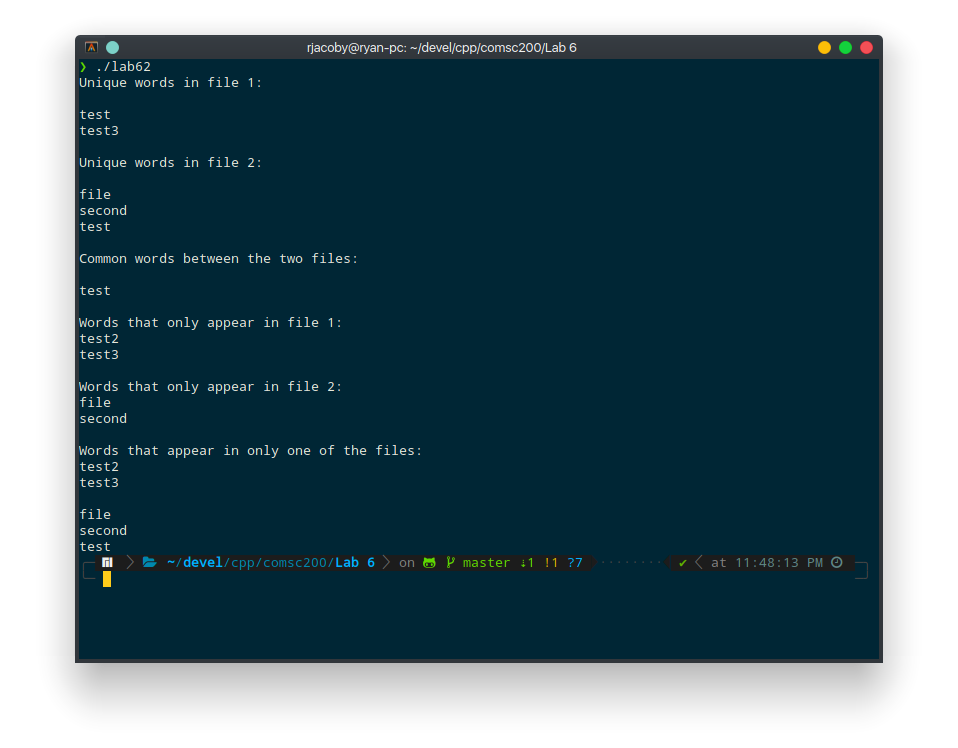
\includegraphics[scale=0.5]{analysis.png}

\section{Word Count}

\begin{lstlisting}[language=c++, caption=main.cpp]
// Ryan Jacoby

#include<iostream>
#include<fstream>
#include<map>
#include<string>

using namespace std;

int main() {
    map<string, int> wc;
    ifstream fin;

    fin.open("input.txt");

    while(fin) {
        string str;
        fin >> str;
        if(wc.count(str) == 0) wc.insert(make_pair(str, 1));
        else wc.at(str)++;
    }

    map<string, int>::iterator it;
    for(it = ++wc.begin(); it != wc.end(); it++) {
        cout << it->first << "\t\t" << it->second << '\n';
    }

    return 0;
}
\end{lstlisting}

\begin{lstlisting}[caption=input.txt]
test test2
test2
test3
test2
\end{lstlisting}

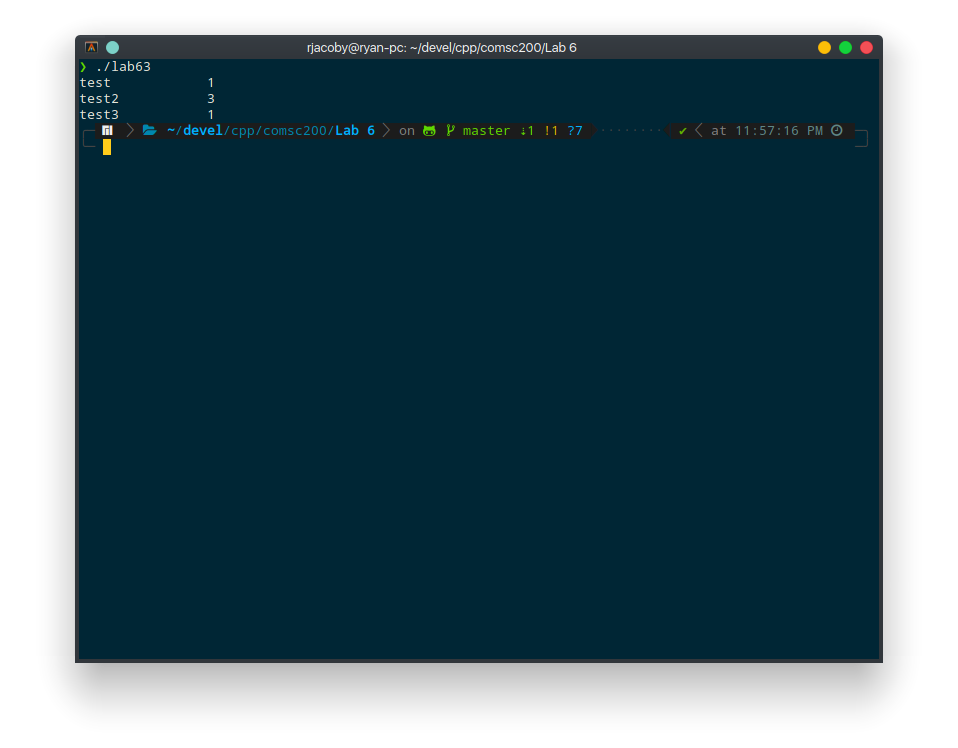
\includegraphics[scale=0.5]{wordcout.png}

\end{document}
